\documentclass[11pt]{article}

\usepackage{amsfonts}
% or
\usepackage{amssymb}
\usepackage{xparse}
\usepackage{amsmath}
\usepackage{physics}
\usepackage{graphicx}
\usepackage[margin=1.2in]{geometry}
\usepackage[colorlinks, linkcolor = cyan, citecolor = cyan, filecolor = cyan, urlcolor = blue]{hyperref} 


\graphicspath{ {./images/} }
%% save grapics in "images" Subfolder
%% do \includegraphics {name} %%(pngs mostly)

\begin{document}



\begin{center}
\textbf{Logische Programmierung, Serie 01}
\end{center}

\begin{flushleft}
Name (Matrikelnummer): \\
Nico Trebbin (218204402)\\
Nils Henrik Seitz (218205308)\\
\end{flushleft}

\begin{flushleft}
Gruppe:	10 \\
Datum: 03.05.2019\\
\end{flushleft}


\begin{flushleft}
\textbf{1}
\end{flushleft}
\begin{flushleft}
 c)
 \end{flushleft} 
\begin{center}
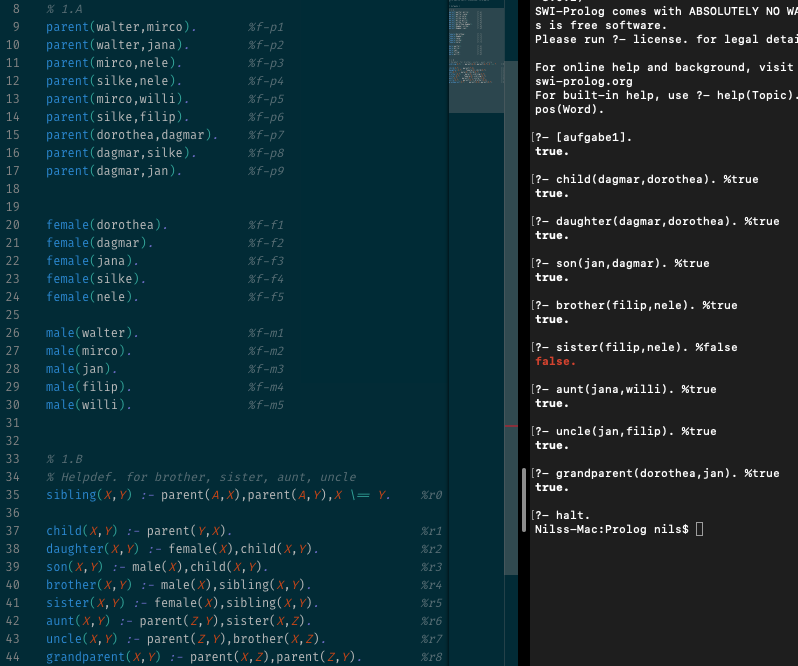
\includegraphics [scale=0.5]{1c}
\end{center}
\newpage
\begin{flushleft}
 d)
 \end{flushleft} 
 \texttt{\underline{brother(X,Y).}\\
 $\Downarrow$ r4 $\lbrace$X=X, Y=Y$\rbrace$\\
 male(X),sibling(X,Y).\\
 $\Downarrow$ f-m1 $\lbrace$X=walter, Y=Y$\rbrace$\\
 male(walter),sibling(walter,Y).\\
 $\Downarrow$ r0 $\lbrace$X=walter, Y=Y, A=A$\rbrace$\\
 male(walter),parent(A,walter),parent(A,Y),walter$\neq$Y.\\
 $\Downarrow$  kein passender Fakt: parent(A,walter)\\
 false. $\Rightarrow$ sibling(walter,Y)  is false $\Rightarrow$ brother(walter,Y) is false. \\
 \\
 male(X),sibling(X,Y).\\
 $\Downarrow$ f-m2 $\lbrace$X=mirco, Y=Y$\rbrace$\\
 male(mirco),sibling(mirco,Y).\\
 $\Downarrow$ r0 $\lbrace$X=mirco, Y=Y, A=A$\rbrace$\\
 male(mirco),parent(A,mirco),parent(A,Y),mirco$\neq$Y. \\
 $\Downarrow$ f-p1 $\lbrace$X=mirco, Y=Y, A=walter$\rbrace$\\
 male(mirco),parent(walter,mirco),parent(walter,Y),mirco$\neq$Y. \\
*  $\Downarrow$ f-p1 $\lbrace$X=mirco, Y=mirco, A=walter$\rbrace$\\
* male(mirco),parent(walter,mirco),parent(walter,mirco),mirco$\neq$mirco. \\
*  $\Downarrow$  mirco=mirco, daher\\
* false. \\
**$\Downarrow$ f-p2 $\lbrace$X=mirco, Y=jana, A=walter$\rbrace$\\
**male(mirco),parent(walter,mirco),parent(walter,jana),mirco$\neq$jana. \\
**$\Downarrow$ mirco$\neq$jana,daher \\
true. $\Rightarrow$ sibling(mirco,jana)  is true $\Rightarrow$ brother(mirco,jana) is true. $\Rightarrow$\\
 X=mirco, Y=jana;\\
\\
male(X),sibling(X,Y).\\
 $\Downarrow$ f-m3 $\lbrace$X=jan, Y=Y$\rbrace$\\
 male(jan),sibling(jan,Y).\\
 $\Downarrow$ r0 $\lbrace$X=jan, Y=Y, A=A$\rbrace$\\
 male(jan),parent(A,jan),parent(A,Y),jan$\neq$Y. \\
 $\Downarrow$ f-p9 $\lbrace$X=jan, Y=Y, A=dagmar$\rbrace$\\
 male(jan),parent(dagmar,jan),parent(dagmar,Y),jan$\neq$Y. \\
* $\Downarrow$ f-p8 $\lbrace$X=jan, Y=silke, A=dagmar$\rbrace$\\
* male(jan),parent(dagmar,jan),parent(dagmar,silke),jan$\neq$silke. \\
* $\Downarrow$  jan$\neq$silke,daher \\
true. $\Rightarrow$ sibling(jan,silke)  is true $\Rightarrow$ brother(jan,silke) is true. $\Rightarrow$\\
X=jan, Y=silke;\\
**$\Downarrow$ f-p9 $\lbrace$X=jan, Y=jan, A=dagmar$\rbrace$\\
**male(jan),parent(dagmar,jan),parent(dagmar,jan),jan$\neq$jan. \\
**jan=jan, daher false. 
\newpage 
\begin{flushleft}
male(X),sibling(X,Y).\\
 $\Downarrow$ f-m4 $\lbrace$X=filip, Y=Y$\rbrace$\\
 male(filip),sibling(filip,Y).\\
 $\Downarrow$ r0 $\lbrace$X=filip, Y=Y, A=A$\rbrace$\\
 male(filip),parent(A,filip),parent(A,Y),filip$\neq$Y. \\
 $\Downarrow$ f-p6 $\lbrace$X=filip, Y=Y, A=silke$\rbrace$\\
 male(filip),parent(silke,filip),parent(silke,Y),filip$\neq$Y. \\
* $\Downarrow$ f-p4 $\lbrace$X=filip, Y=nele, A=silke$\rbrace$\\
* male(filip),parent(silke,filip),parent(silke,nele),filip$\neq$nele. \\
* $\Downarrow$  filip$\neq$nele,daher \\
true. $\Rightarrow$ sibling(filip,nele)  is true $\Rightarrow$ brother(filip,nele) is true. $\Rightarrow$\\
X=filip, Y=nele;\\
**$\Downarrow$ f-p6 $\lbrace$X=filip, Y=filip, A=silke$\rbrace$\\
**male(filip),parent(silke,filip),parent(silke,filip),filip$\neq$filip. \\
**filip=filip, daher false.
\end{flushleft}
\begin{flushleft}
male(X),sibling(X,Y).\\
 $\Downarrow$ f-m5 $\lbrace$X=willi, Y=Y$\rbrace$\\
 male(willi),sibling(willi,Y).\\
 $\Downarrow$ r0 $\lbrace$X=willi, Y=Y, A=A$\rbrace$\\
 male(willi),parent(A,willi),parent(A,Y),filip$\neq$Y. \\
 $\Downarrow$ f-p5 $\lbrace$X=willi, Y=Y, A=mirco$\rbrace$\\
 male(willi),parent(mirco,willi),parent(mirco,Y),willi$\neq$Y. \\
* $\Downarrow$ f-p3 $\lbrace$X=willi, Y=nele, A=mirco$\rbrace$\\
* male(willi),parent(mirco,willi),parent(mirco,nele),willi$\neq$nele. \\
* $\Downarrow$  willi$\neq$nele,daher \\
true. $\Rightarrow$ sibling(willi,nele)  is true $\Rightarrow$ brother(willi,nele) is true. $\Rightarrow$\\
X=willi, Y=nele;\\
**$\Downarrow$ f-p5 $\lbrace$X=willi, Y=willi, A=mirco$\rbrace$\\
**male(willi),parent(mirco,willi),parent(mirco,willi),willi$\neq$willi. \\
**willi=willi, daher false.
\end{flushleft}
 }  
 \texttt{ \begin{flushleft} \underline{sister(X,Y).}\\
 $\Downarrow$ r5 $\lbrace$X=X, Y=Y$\rbrace$\\
 female(X),sibling(X,Y).\\
 $\Downarrow$ f-f1 $\lbrace$X=dorothea, Y=Y$\rbrace$\\
 female(dorothea),sibling(dorothea,Y).\\
 $\Downarrow$ r0 $\lbrace$X=dorothea, Y=Y, A=A$\rbrace$\\
 female(dorothea),parent(A,dorothea),parent(A,Y),dorothea$\neq$Y.\\
 $\Downarrow$  kein passender Fakt: parent(A,dorothea)\\
 false. $\Rightarrow$ sibling(dorothea,Y)  is false $\Rightarrow$ sister(dorothea,Y) is false. \\
 \end{flushleft}
 \newpage
 \begin{flushleft}
 female(X),sibling(X,Y).\\
 $\Downarrow$ f-m2 $\lbrace$X=dagmar, Y=Y$\rbrace$\\
 female(dagmar),sibling(dagmar,Y).\\
 $\Downarrow$ r0 $\lbrace$X=dagmar, Y=Y, A=A$\rbrace$\\
 female(dagmar),parent(A,dagmar),parent(A,Y),dagmar$\neq$Y. \\
 $\Downarrow$ f-p7 $\lbrace$X=dagmar, Y=Y, A=dorothea$\rbrace$\\
 female(dagmar),parent(dorothea,dagmar),parent(dorothea,Y),dagmar$\neq$Y. \\
$\Downarrow$ f-p7 $\lbrace$X=dagmar, Y=dagmar, A=dorothea$\rbrace$\\
female(dagmar),parent(dorothea,dagmar),parent(dorothea,dagmar),dagmar$\neq$dagmar. \\
$\Downarrow$  dagmar=dagmar, daher\\
 false. $\Rightarrow$ sibling(dagmar,Y)  is false $\Rightarrow$ sister(dagmar,Y) is false. \\
 \end{flushleft}
 \begin{flushleft}
 female(X),sibling(X,Y).\\
 $\Downarrow$ f-m3 $\lbrace$X=jana, Y=Y$\rbrace$\\
 female(jana),sibling(jana,Y).\\
 $\Downarrow$ r0 $\lbrace$X=jana, Y=Y, A=A$\rbrace$\\
 female(jana),parent(A,jana),parent(A,Y),jana$\neq$Y. \\
 $\Downarrow$ f-p2 $\lbrace$X=jana, Y=Y, A=walter$\rbrace$\\
 female(jana),parent(walter,jana),parent(walter,Y),jana$\neq$Y. \\
* $\Downarrow$ f-p1 $\lbrace$X=jana, Y=mirco, A=walter$\rbrace$\\
* female(jana),parent(walter,jana),parent(walter,mirco),jana$\neq$mirco. \\
* $\Downarrow$ jana$\neq$mirco,daher \\
true. $\Rightarrow$ sibling(jana,mirco)  is true $\Rightarrow$ sister(jana,mirco) is true. $\Rightarrow$\\
X=jana, Y=mirco;\\
**$\Downarrow$ f-p2 $\lbrace$X=jana, Y=jana, A=walter$\rbrace$\\
**female(jana),parent(walter,jana),parent(walter,jana),jana$\neq$jana. \\
**jana=jana, daher false.
 \end{flushleft} 
  \begin{flushleft}
 female(X),sibling(X,Y).\\
 $\Downarrow$ f-m4 $\lbrace$X=silke, Y=Y$\rbrace$\\
 female(silke),sibling(silke,Y).\\
 $\Downarrow$ r0 $\lbrace$X=silke, Y=Y, A=A$\rbrace$\\
 female(silke),parent(A,silke),parent(A,Y),silke$\neq$Y. \\
 $\Downarrow$ f-p8 $\lbrace$X=silke, Y=Y, A=dagmar$\rbrace$\\
 female(silke),parent(dagmar,silke),parent(dagmar,Y),silke$\neq$Y. \\
* $\Downarrow$ f-p8 $\lbrace$X=silke, Y=silke, A=dagmar$\rbrace$\\
* female(silke),parent(dagmar,silke),parent(dagmar,silke),silke$\neq$silke. \\
* jana=jana, daher false.\\
**$\Downarrow$ f-p9 $\lbrace$X=jana, Y=jan, A=walter$\rbrace$\\
**female(silke),parent(dagmar,silke),parent(dagmar,jan),silke$\neq$jan. \\
**$\Downarrow$ silke$\neq$jan,daher \\
true. $\Rightarrow$ sibling(silke,jan)  is true $\Rightarrow$ sister(silke,jan) is true. $\Rightarrow$\\
X=silke, Y=jan;
 \end{flushleft} 
 \newpage
 \begin{flushleft}
 female(X),sibling(X,Y).\\
 $\Downarrow$ f-m5 $\lbrace$X=nele, Y=Y$\rbrace$\\
 female(nele),sibling(nele,Y).\\
 $\Downarrow$ r0 $\lbrace$X=nele, Y=Y, A=A$\rbrace$\\
 female(nele),parent(A,nele),parent(A,Y),nele$\neq$Y. \\
' $\Downarrow$ f-p3 $\lbrace$X=nele, Y=Y, A=mirco$\rbrace$\\
' female(nele),parent(mirco,nele),parent(mirco,Y),nele$\neq$Y. \\
' * $\Downarrow$ f-p3 $\lbrace$X=nele, Y=nele, A=mirco$\rbrace$\\
' * female(nele),parent(mirco,nele),parent(mirco,nele),nele$\neq$nele. \\
' * nele=nele, daher false.\\
' **$\Downarrow$ f-p6 $\lbrace$X=nele, Y=willi, A=mirco$\rbrace$\\
' **female(nele),parent(mirco,nele),parent(mirco,willi),nele$\neq$willi. \\
' **$\Downarrow$ nele$\neq$willi,daher \\
true. $\Rightarrow$ sibling(nele,willi)  is true $\Rightarrow$ sister(nele,willi) is true. $\Rightarrow$\\
X=nele, Y=willi;\\
''$\Downarrow$ f-p4 $\lbrace$X=nele, Y=Y, A=silke$\rbrace$\\
''female(nele),parent(silke,nele),parent(silke,Y),nele$\neq$Y. \\
''* $\Downarrow$ f-p4 $\lbrace$X=nele, Y=nele, A=silke$\rbrace$\\
''* female(nele),parent(silke,nele),parent(silke,nele),nele$\neq$nele. \\
''* nele=nele, daher false.\\
''**$\Downarrow$ f-p6 $\lbrace$X=nele, Y=filip, A=silke$\rbrace$\\
''**female(nele),parent(silke,nele),parent(silke,filip),nele$\neq$filip. \\
''**$\Downarrow$ nele$\neq$filip,daher \\
true. $\Rightarrow$ sibling(nele,filip)  is true $\Rightarrow$ sister(nele,filip) is true. $\Rightarrow$\\
X=nele, Y=filip;
 \end{flushleft} 
 }
\end{document}